\documentclass{article}
\usepackage[x11names, svgnames, rgb]{xcolor}

% Language setting
% Replace `english' with e.g. `spanish' to change the document language
\usepackage[english]{babel}

% Set page size and margins
% Replace `letterpaper' with `a4paper' for UK/EU standard size
\usepackage[letterpaper,top=2cm,bottom=2cm,left=3cm,right=3cm,marginparwidth=1.75cm]{geometry}

% Useful packages
\usepackage{amsmath}
\usepackage{graphicx}
\usepackage{url}
\usepackage[colorlinks=true, allcolors=blue]{hyperref}

\usepackage{tikz}
\usetikzlibrary{snakes,arrows,shapes}

%\title{KnowTeX: A \LaTeX-Based Tool for Visualizing Mathematical Dependencies}
\title{KnowTeX: Visualizing Mathematical Dependencies}
\author{Elif Uskuplu \and Lawrence S.~Moss \and Valeria de Paiva}

\begin{document}
\maketitle

\begin{abstract}
Mathematical knowledge exists in many forms, ranging from informal textbooks and lecture notes to large formal proof
libraries, yet moving between these representations remains difficult. Informal texts hide dependencies, while formal
systems expose every detail in ways that are not always human-readable. Dependency graphs offer a middle ground
by making visible the structure of results, definitions, and proofs. We present KnowTeX, a standalone, user-friendly tool that extends the ideas of Lean’s Blueprints, enabling the visualization of conceptual dependencies directly from
\LaTeX\ sources. Using a simple {\verb|\uses|} command, KnowTeX extracts relationships among statements and generates
previewable graphs in DOT and TikZ formats. Applied to mathematical texts, such graphs clarify core results, support
education and formalization, and provide a resource for aligning informal and formal mathematical representations.
We argue that dependency graphs should become a standard feature of mathematical writing, benefiting both human
readers and automated systems.
\end{abstract}

\section{Introduction}

Mathematical writing is inherently complex. Definitions, theorems, and proofs form dense networks of interdependent ideas, where results often build on earlier ones in subtle and intertwined ways. In textbooks and lecture notes, these connections are spread across multiple chapters and sections, making it difficult to perceive the overall structure of the knowledge being presented. 
The richness of mathematical discourse, while essential for depth and rigor, also creates challenges for navigation, comprehension, and reuse of information.

In contrast, formal proof assistants such as Lean (\cite{demoura2015}), Agda (\cite{norell2009}), or Rocq\footnote{Formerly known as Coq.} (\cite{bertot2010}) make every dependency explicit. When a mathematical theory is formalized, each proof must declare precisely which results it uses, since omitting even a single dependency would render the proof invalid. These systems, therefore, expose the finest level of detail in mathematical relationships, capturing the complete web of definitions, lemmas, and theorems in code.
However, this level of detail--while powerful for verification--can be overwhelming for humans, as it demands close familiarity with the entire formal environment.

Between the implicit structure of informal texts and the exhaustive precision of formal systems lies a useful middle ground: dependency graphs. A dependency graph represents mathematical statements as nodes and their conceptual or logical relationships as edges, providing a readable overview of how results depend on one another. Such visualizations make the structure of a text more transparent without requiring formalization, offering both researchers and educators a practical way to explore, analyze, and align mathematical knowledge.

Some tools have already explored ways to generate dependency graphs from mathematical documents. One notable example is Patrick Massot’s `Lean Blueprint'\footnote{Code in \url{https://github.com/PatrickMassot/leanblueprint}})  system, which extends the concept of dependency between components of a proof by linking informal mathematical text with other corresponding formal proofs in the Lean theorem prover. Another similar tool is plasTeXdepgraph\footnote{See \url{https://github.com/PatrickMassot/plastexdepgraph})}, a simplified version of the Lean blueprint, a plugin for plasTeX.
%(Rush et al., 2006) framework: plasTeXdepgraph
This simply removes the connection to the Lean prover, still linking informal mathematical text in plasTeX to interactive dependency graphs. Together, these tools demonstrate the value of dependency graphs for understanding mathematical structure, though they remain closely tied to specific technical ecosystems.

Another related approach is the recently-introduced `Trouver' system\footnote{See \url{https://github.com/hyunjongkimmath/trouver}.}, which applies machine learning to automatically infer dependency structures from \LaTeX\ documents. 
Unlike tools that rely on explicit markup commands, Trouver allows users to simply upload a \LaTeX file, and it generates a dependency graph using statistical and linguistic models. This approach removes the manual effort required to annotate dependencies, offering a convenient and automated workflow. 
However, its effectiveness depends strongly on the clarity of the source text: when relationships are implicit or linguistically complex, the model may miss important links or produce spurious ones, resulting in overly dense or incomplete graphs. Trouver thus
represents a promising yet imperfect data-driven alternative, practical for quick visualization but less reliable for precise structural analysis.
%
There is also a recent commercial service `ScienceStack'\footnote{See \url{http://www.sciencestack.ai}.} that provides HTML rendering as well as dependency graphs for the user's \LaTeX\ papers, for a price and using closed source software.

In this work, we introduce KnowTeX, a lightweight and user-friendly tool for generating dependency graphs directly from \LaTeX sources. Conceptually, KnowTeX follows the same principles as plasTeXdepgraph and the tool Lean Blueprint, using explicit markup to indicate relationships among statements.
However, unlike systems integrated into broader ecosystems or relying on machine learning, KnowTeX focuses purely on the structure expressed within the text itself. 
Authors can specify connections by inserting simple \LaTeX commands such as {\verb|\uses{...}|}, from which the program automatically builds a dependency graph. 
The tool operates independently—no external framework, theorem prover, or AI model is required—and outputs graphs in standard DOT and TikZ formats. 
By emphasizing transparency and simplicity, KnowTeX aims to make dependency visualization accessible to anyone working with mathematical documents, bridging the gap between readability and formal precision.

Our goal here is not only to introduce KnowTeX as an independent tool, but also to highlight the broader role that dependency graphs could play in mathematical communication. 
We focus on how such graphs can serve as a standard resource for organizing, teaching, and formalizing mathematical knowledge. Through comparisons with existing systems such as  Lean Blueprint, plasTeXdepgraph, and the machine learning based Trouver, we discuss the strengths and limitations of each approach and show how KnowTeX extends this line of work in a simpler, more accessible direction. Ultimately, we argue that dependency graphs deserve to become a standard component of mathematical writing, benefiting both human understanding and automated reasoning.


%Artificial Intelligence Disclosure. Portions of the English text and parts of the Python implementation were developed with the assistance of generative AI tools (OpenAI’s GPT-5). These tools were used only for language polishing and coding support under the authors’ supervision; all ideas, design choices, and evaluations are the sole responsibility of the authors.

\section{Dependency graphs}
%The Role of Dependency Graphs
A natural starting point for understanding the value of dependency graphs lies in their simplest application: supporting human learning. 
Dependency graphs serve a practical role in navigating and learning mathematical material. Beyond illustrating conceptual structure, they help readers plan efficient study paths and identify the minimal background required for a given result. 
In our case study based on Tom Leinster’s `Basic Category Theory' \cite{leinster2014}, a graph mapping definitions, lemmas, and propositions makes it clear which earlier concepts support key theorems such as the Yoneda Lemma or the Adjoint Functor Theorem. Rather than reading linearly from the beginning, a learner can focus
on the relevant portion of the conceptual network, reducing cognitive load and saving time.

Dependency graphs also play a crucial role in the technical side of mathematical formalization. 
When formalizing a theory within a proof assistant, efficiency often depends on identifying exactly which concepts and results are required for a particular proof. 
A dependency graph provides a clear map of these relationships, allowing researchers to include only the necessary components while omitting unrelated material. 
Although fully formalizing every result in a textbook can be an ideal long-term goal, in practice it is more efficient to formalize selectively -- focusing on the minimal set of definitions and lemmas needed for a given theorem. 
This selective approach reduces both computational load and human effort, as shorter, more focused formalizations are easier to maintain and verify. 
In this way, dependency graphs help optimize the design and scalability of formal libraries, supporting faster and more resource-efficient proof development.

Dependency graphs can also contribute to the construction of machine learning datasets and structured mathematical corpora. The need for such datasets and math corpora has been discussed by several people, e.g., de Paiva and Fong \cite{fong2021}, Collard et al \cite{collard2024}, Welleck et al \cite{welleck2021}. 
There are initiatives to compile a large-scale, machine-readable collection of articles in research mathematics, starting with category theory abstracts from the journal Theory and Applications of Categories\footnote{\url{https://github.com/ToposInstitute/tac-corpus}}, enabling the study of mathematical language and concept extraction for large language models \cite{depaiva2023}. 

One of the major challenges in such work is ensuring that all relevant concepts and their interrelations are accurately captured. Missing definitions, unlinked results, or redundant statements can limit the dataset’s usefulness for both linguistic and logical analysis. 
By providing an explicit representation of how mathematical statements depend on one another, dependency graphs can help detect these issues and guide curation.
They offer a principled way to align informal mathematical writing with formal structures, improving both dataset quality and interpretability for AI-driven research in mathematics.
In summary, dependency graphs serve as versatile tools that reveal the structure of mathematical knowledge at multiple levels, from supporting individual learning to guiding formalization and lexicon/corpus construction. 
Their ability to make conceptual relationships explicit allows both humans and machines to navigate mathematics more effectively.

To explore one concrete way of generating such graphs, the next section introduces KnowTeX, our standalone tool designed to create dependency graphs directly from \LaTeX documents in a simple and transparent manner.


\section{KnowTex}

KnowTeX\footnote{See \url{https://github.com/ElifUskuplu/KnowTex}.} is a standalone Python application that generates dependency graphs directly from \LaTeX\ sources. 
The program takes a single \LaTeX\ file as input and produces two main outputs: a DOT file and a TikZ-based \LaTeX\ file representing the same graph. 
The DOT file is a standard Graphviz format that can be rendered or made interactive using external visualization tools, such as Graphviz\footnote{\url{https://graphviz.org/}} or viz.js\footnote{\url{https://viz.js.org/}}, making it suitable for integration into HTML pages or online repositories. 
%
The TikZ\footnote{\url{https://tikz.dev/}} file provides a static version of the graph that can be included directly in \LaTeX\ documents or exported as a PDF.
Before producing these outputs, KnowTeX offers a preview feature within the application interface, allowing users to inspect the generated graph visually.

The design of KnowTeX emphasizes both flexibility and control for the user. After loading a \LaTeX\ source file, the user specifies which types of mathematical environments should be scanned by the program. 

Commonly recognized environments include `Definition', `Theorem', `Lemma', `Proposition', `Corollary', `Construction', `Example', and `Remark'. 
These can be selected individually or collectively, depending on the desired level of detail. 
To accommodate variations in authoring styles, KnowTeX also supports multiple naming conventions through regular expressions, for example, recognizing shortened forms such as “thm” or “def” as valid environments.
When a document contains multiple chapters, the user can choose to analyze the entire text or focus on a specific chapter, allowing for localized graph generation and more targeted exploration. 
Once the selections are made, the program automatically scans the specified environments, preparing the data for dependency extraction and graph construction as described below.

To construct the dependency graph, KnowTeX relies on a lightweight command-based linking system embedded within the \LaTeX\ source. We illustrate the procedure for introducing dependencies in KnowTeX with a simple example. The author writes standard mathematical environments in \LaTeX\, assigns labels in the usual way, and records dependencies by inserting the \verb|\uses| command.

\begin{quote}
\begin{verbatim}
\begin{definition}\label{def:ring}
A ring is a set with two operations satisfying ...
\end{definition}

\begin{lemma}\label{lem:ring-unit}
\uses{def:ring}
In a ring, if $1=0$ then every element is zero.
\end{lemma}

\begin{proof}
Trivial from the axioms.
\end{proof}

\begin{corollary}\label{cor:trivial-ring}
\uses{def:ring}
If a ring satisfies $1 = 0$, then it is the trivial ring $\{0\}$.
\end{corollary}

\begin{proof}
\uses{lem:ring-unit}
By Lemma~\ref{lem:ring-unit}, if $1 = 0$, then every element equals $0$.  
Hence, the ring contains only one element, $0$, and is therefore the trivial ring.
\end{proof}
\end{verbatim}
\end{quote}

From this annotated source, KnowTeX extracts labeled mathematical objects and their declared dependencies. When the \verb|\uses| command appears inside the statement of a definition, lemma, or corollary, it records a conceptual dependency; in the generated graph, this relation is visualized with a dashed edge. When it appears inside a proof environment, it records a direct logical dependency arising from the proof itself, represented by a solid edge. Running KnowTeX on the example above produces the following TikZ graph:

\begin{center}
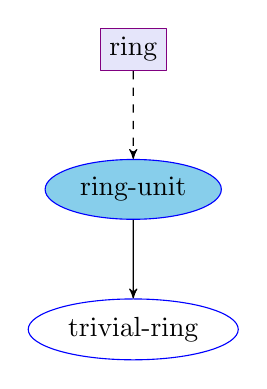
\begin{tikzpicture}[scale=0.7, >=latex',line join=bevel,]
%%
\node (def_ring) at (60.445bp,162.0bp)
  [draw=Purple,fill=Lavender,rectangle] {ring};
\node (lem_ring-unit) at (60.445bp,90.0bp)
  [draw=Blue,fill=SkyBlue,ellipse] {ring-unit};
\node (cor_trivial-ring) at (60.445bp,18.0bp)
  [draw=Blue,fill=White,ellipse] {trivial-ring};

\draw [-stealth',dashed]
  (def_ring) .. controls (60.445bp,135.98bp) and (60.445bp,126.71bp)
  .. (lem_ring-unit);

\draw [-stealth']
  (lem_ring-unit) .. controls (60.445bp,63.983bp) and (60.445bp,54.712bp)
  .. (cor_trivial-ring);
\end{tikzpicture}
\end{center}


The resulting graph contains a node for the definition of a ring, a node for the lemma, and a node for the corollary. The dashed edge from the definition node to the lemma node represents a conceptual dependency declared in the lemma statement. The solid edge from the lemma node to the corollary node represents a logical dependency declared in the proof of the corollary. KnowTeX computes the transitive closure of the dependency relation when constructing the graph. For this reason, although the corollary conceptually depends on the definition of a ring, no additional dashed edge from the definition node to the corollary node is drawn. This dependency is already implied by the path through the lemma, and omitting the redundant edge keeps the visualization readable while preserving the full dependency information.

In addition to the {\verb|\uses |} command, KnowTeX supports an optional {\verb|\proves |} command, used when the link between a proof and its corresponding statement cannot be inferred automatically, for example, when intervening remarks or text interrupt the expected structure. 
In such cases, {\verb|\proves |} explicitly declares which labeled theorem or lemma is being proved, ensuring that all dependencies are correctly represented in the resulting graph. 

 \begin{figure}[h!]
 \centering
  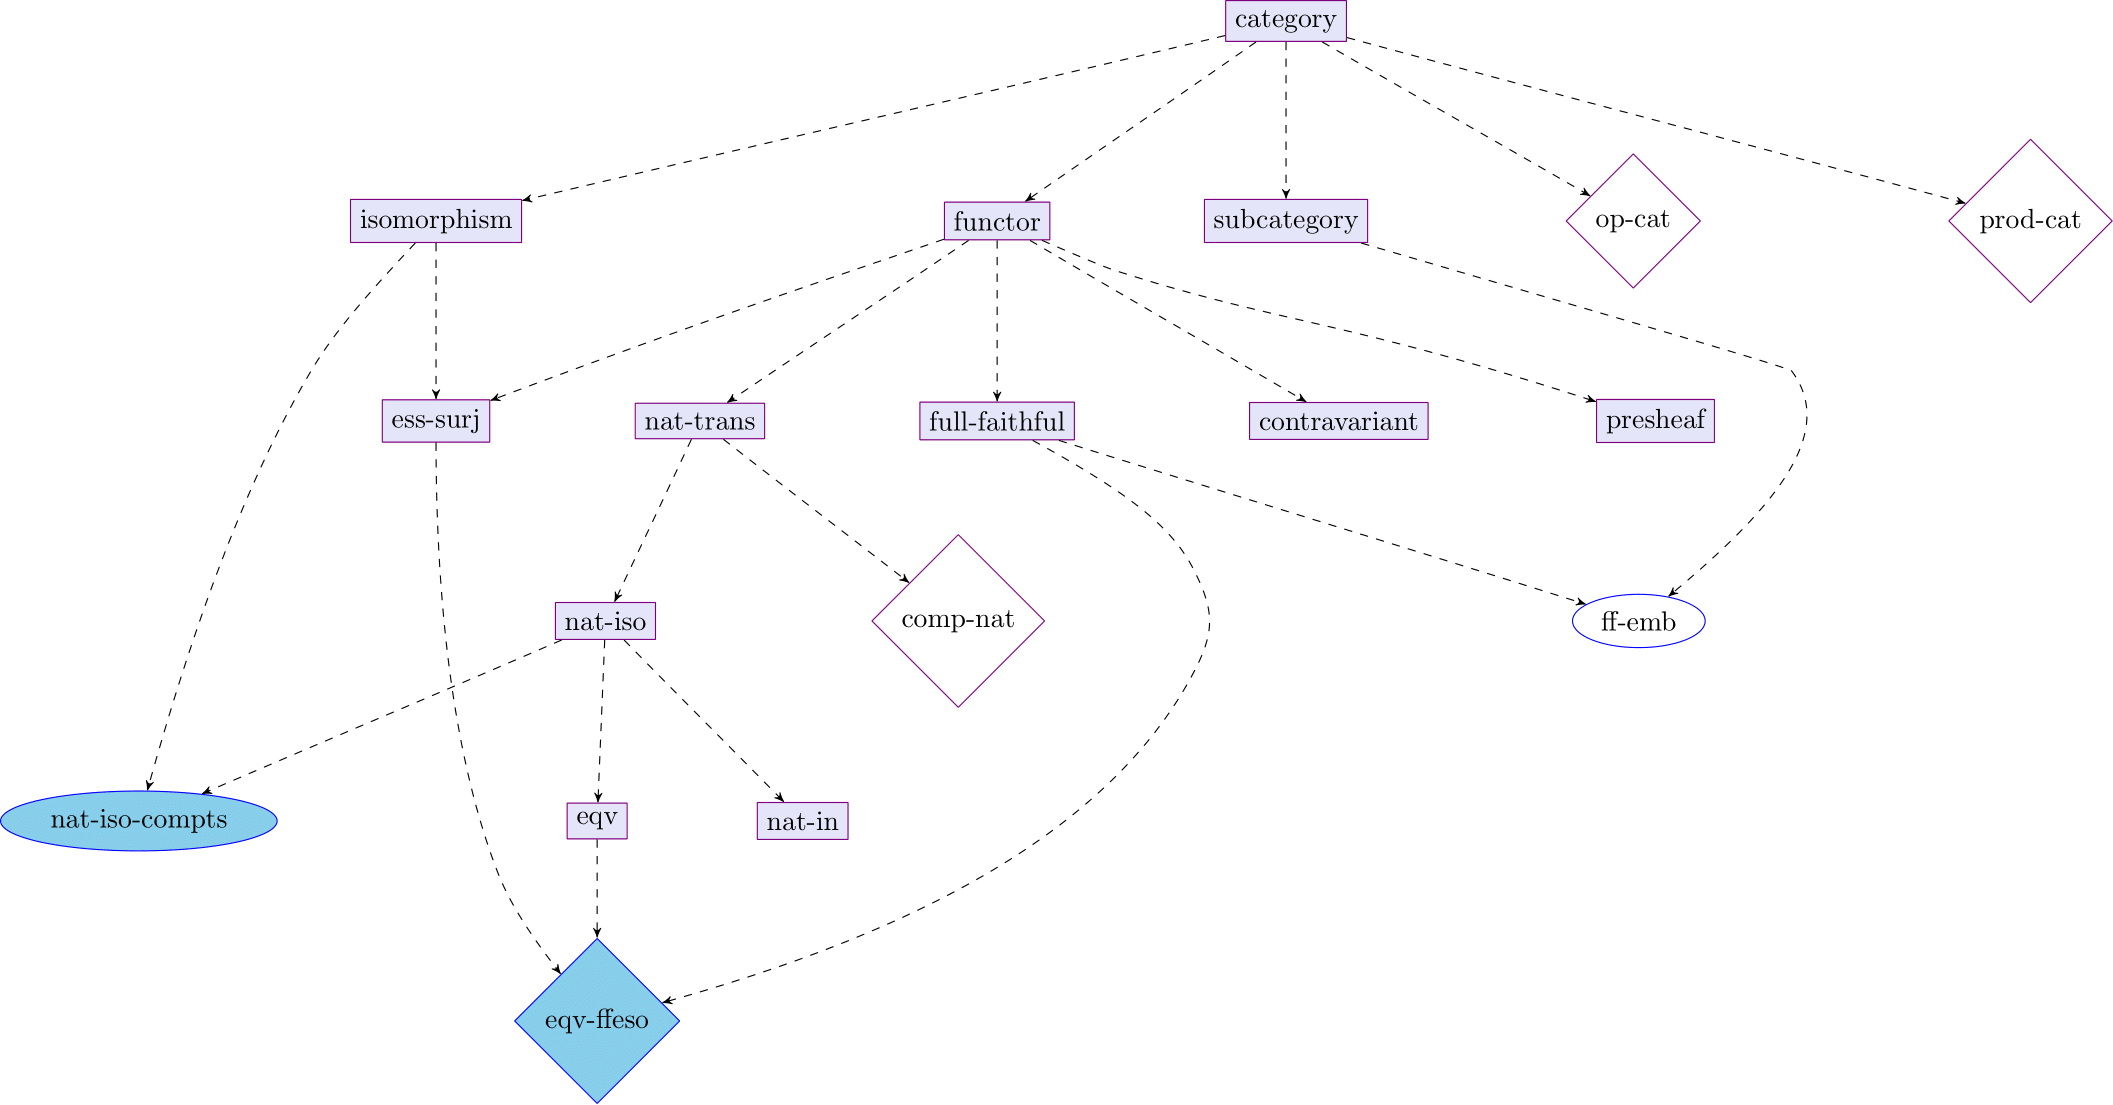
\includegraphics[width=0.5\textwidth]{ch1-graph.png}
 \caption{The dependency graph of Chapter 1 of Leinster's `Basic Category Theory'}
 \end{figure}
In Figure 1, the graph is extracted from the first chapter of \textit{Basic Category Theory} by Leinster. 
In this graph, boxes represent definitions, white diamonds constructions, blue diamonds propositions, and ellipses lemmas.
Additional chapters and examples involving more
environments are provided in the GitHub repository of the program.




The most influential system for representing mathematical dependencies is Lean’s `Blueprint', which provides structured links between informal text and formal proof code. 
Building on this idea, KnowTeX extends the same command logic to the broader \LaTeX\ ecosystem while remaining independent of any specific proof assistant. 
It can thus be viewed as an agnostic blueprint tool that could complement frameworks such as Lean, Rocq, Isabelle, or Agda. 
The command system in KnowTeX follows the same underlying structure of Massot’s plasTeXdepgraph plugin, which the Lean Blueprint relies on for graph generation. 
This deliberate compatibility ensures that \LaTeX\ documents prepared for either system can
be processed directly by KnowTeX without modification, yielding consistent dependency relations.

We verified this compatibility across several case studies, confirming that KnowTeX reproduces the same dependency mappings as these earlier tools while offering a more streamlined, user-oriented workflow.
PlasTeX\footnote{See \url{https://plastex.github.io/plastex/}.} is a Python package that processes \LaTeX\ documents into an XML-DOM–like object, which can then be used to generate various types of output, including HTML and Braille.
The plasTeXdepgraph plugin compiles \LaTeX\ files into an HTML format that integrates the dependency graph directly into the rendered document, allowing users to click on nodes and navigate to the corresponding results. 
This interactivity is effective when the \LaTeX\ source is written for plasTeX, but compiling legacy or complex documents, those with custom macros or nonstandard environments, can be challenging. 
In our experiments with Tom Leinster’s Basic Category Theory (\cite{leinster2014}), successful compilation required extensive editing and removal of non-essential macros. The Lean Blueprint system extends this HTML-based foundation by connecting dependency graphs with formal proof development, using visual cues to indicate proof status and links to both \LaTeX\ and Lean sources. 
These features are powerful but Lean-centered and presuppose an existing formalization.

In contrast, KnowTeX isolates and simplifies this functionality. 
It focuses solely on dependency visualization, requiring no external ecosystem, HTML conversion, or formal proof integration. 
Like plasTeX, it allows color and shape customization, but through a lightweight, standalone interface that makes dependency analysis accessible to authors and researchers seeking to understand or present the structure of mathematical texts without entering a formal workflow.

The Trouver\footnote{\url{https://github.com/hyunjongkimmath/trouver}} system takes a machine-learning approach to extracting dependency information from \LaTeX\ sources. 
Unlike KnowTeX, which relies on explicit commands, Trouver infers relationships automatically from textual and structural patterns. This automation makes it attractive for large-scale or legacy corpora. But it also makes it less predictable: inferred links may miss subtle logical dependencies or introduce spurious ones. 
KnowTeX, by contrast, prioritizes explicit author control and reproducibility over automation, providing a complementary rather than competing model.

These comparisons illustrate how KnowTeX occupies a distinct position within the existing ecosystem: it preserves compatibility with established tools while remaining lightweight, independent, and focused solely on the visualization of the logical structure. 
%%%%%%
We should also remark that while our experiments and code are geared towards mathematical research text, most of the so-called hard sciences could, perhaps,  benefit from a tool like  KnowTex. \LaTeX\ is used by physicists, chemists, biologists,  etc, and the logical dependency trees that KnowTex makes explicit should be beneficial to these other sciences too.
We turn to the broader implications of this approach and outline possible directions for future development.

\section{Future work}
Beyond the current version, several directions
remain open for extending both KnowTeX and the
broader use of dependency graphs in mathematical
writing:

\noindent {\textbf{Expanding case studies:}} Future work will involve applying KnowTeX to a wider variety of mathematical texts and educational materials. Demonstrating its usefulness across different writing styles and domains will help establish the practical value
of dependency graphs and support their adoption
as a writing standard.

\noindent {\textbf{AI-assisted command generation:}} Inspired by systems such as Trouver, one possible enhancement would be to automate the insertion of {\verb|\uses|}
and {\verb|\proves|} commands through AI-based text
analysis. Such a feature could reduce authors’
manual workload while preserving accuracy and
alignment with the original text structure in addition
to other dependency graph tools.

\noindent {\textbf{Greater interactivity and customization:}} The visualization could be made more dynamic by allowing users to define every graphical parameter from color schemes and node shapes to edge styles directly within the interface. Additionally,
the preview window could evolve into an interactive
display, enabling users to click nodes that link back
to corresponding definitions or theorems within the
compiled PDF.

\noindent {\textbf{Integration with large-scale corpora:}} In large mathematical corpora, dependency graphs can serve as structured metadata, recording which results depend on which definitions. Such metadata enable corpus-level querying, visualization, and linking between informal and formal representations. 
Integrating KnowTeX within corpus-building pipelines would make it possible to study the structure of mathematical theories at scale, supporting both formalization and machine learning research.

These extensions point toward a future in which dependency graphs are not only a visualization aid but an integral part of how mathematical knowledge is written, shared, and explored.

\section{Conclusion}

In  summary, our motivation for developing Know-TeX as an independent, \LaTeX-oriented tool stems from a desire to make dependency graphs a standard element of mathematical writing. Authors already rely on \LaTeX’s label–reference system when structuring their definitions, theorems, and proofs; KnowTeX simply extends this workflow by allowing
them to record the logical connections among these labeled elements through lightweight commands such as {\verb|\uses|}. 

By embedding these relationships directly into the writing process, authors can automatically generate graphical summaries of their work adding, for instance, a dependency graph at the end of each paper or at the conclusion of every chapter in a textbook. 
This integration preserves the author’s natural writing habits while making the conceptual structure of the text explicit and accessible. 
In this sense, KnowTeX aims not to replace existing online or formal systems, but to complement them by enriching the final \LaTeX\ output itself with visual representations of mathematical knowledge.

\bibliographystyle{alpha}
\bibliography{references}

\end{document}
